\documentclass[../main.tex]{subfiles}
\usepackage[utf8]{inputenc}
\usepackage[T1]{fontenc}
\usepackage{graphicx}
\usepackage{longtable}
\usepackage{wrapfig}
\usepackage{rotating}
\usepackage[normalem]{ulem}
\usepackage{amsmath}
\usepackage{amssymb}
\usepackage{capt-of}
\usepackage{hyperref}
\usepackage{float}
\graphicspath{{../}}
\author{Cezary Wieczorkowski}
\date{\today}
\title{Koncepcja}
\hypersetup{
 pdfauthor={Cezary Wieczorkowski},
 pdftitle={Koncepcja},
 pdfkeywords={},
 pdfsubject={},
 pdflang={Polish}}
\begin{document}


\section{Koncepcja nowego stanowiska}

\subsection{Założenia projektowe}

    Po przeanalizowaniu poprzedniego zestawu laboratoryjnego wypracowano następujące założenia dla projektu nowego zestawu:
    \begin{itemize}
    \item Zestaw musi zachować bloki funkcjonalne oraz zasadę działania poprzedniego zestawu.
    \item Zestaw ma zachować tryby pracy: cykl, mikrocykl oraz program.
    \item Zestaw musi emulować komponenty rzeczywistego układu szyny danych.
    \item Zestaw musi umożliwiać łatwą naprawę błędów w jego funkcjonowaniu oraz rozbudowę o nowe funkcjonalności.
    \item Zestaw musi zachować przejrzysty sposób wizualizacji stanu poszczególnych komponentów.
    \item Zestaw musi posiadać uniwersalny interfejs użytkownika pozwalający na łatwą obsługę zestawu oraz późniejsze jego modyfikacje.
    \end{itemize}

\subsection{Projekt sprzętowy}

    \subsubsection{Wybór mikrokontrolera}

    Ze względu na wybrane podejście symulacji programowej działania układu szyny danych, mikrokontroler jest centralnym elementem budowanego układu.
    W celu zapewnienia możliwości dalszej rozbudowy oraz wprowadzania poprawek do układu musi być to nowoczesna i łatwo dostępna platforma. 
    Istniejąca wersja zestawu jest oparta o mikrokontroler Atmega 8 oraz Atmega 32. Są to urządzenia pracujące z częstotliwością 16 MHz oraz 
    posiadające odpowiednio 1 Kb oraz 2 Kb pamięci RAM \cite{at:atmega8} \cite{at:atmega32}. Większość mikrokontrolerów dostępnych obecnie na 
    rynku oferuje znacząco większe możliwości. 
    \par
    Jako mikrokontroler do budowy zestawu wybrano układ RP2040 firmy Rassbery Pi \cite{rp:rp2040} obecny na płytce rozwojowej Rassbery Pi Pico. 
    Jest to układ oparty o architekturę ARM Cortex M0+, posiada 264 Kb pamięci RAM oraz pracuje z częstotliwością 133 MHz. Układ posiada duży zapas
    zasobów sprzętowych co pozwoli na szerokie możliwości rozbudowy zestawu w przyszłości. Dodatkowo dostępność układu na płytce rozwojowej uprości
    proces budowy sprzętowej części zestawu gdyż płytka ta zawiera wszystkie elementy niezbędne do pracy mikrokontrolera.

    \subsubsection{Elementy interfejsu użytkownika}

    Interfejs użytkownika zestawu powinien umożliwiać łatwą obsługę zestawu oraz umożliwiać łatwe wprowadzenie zmian w jego strukturze. Takie wymagania
    najlepiej spełni interfejs oparty o wyświetlacz wyświetlający menu z opcjami do wyboru oraz interfejs do nawigacji pomiędzy nimi. 
    Jako wyświetlacz zdecydowano się zastosować wyświetlacz znakowy LCD 20x4. Jest to wyświetlacz oparty o popularny układ sterujący HD44780 \cite{lcd_hd44780}.
    Dzięki prostocie obsługi oraz długiej obecności na rynku tego typu wyświetlacze są wspierane przez bardzo szeroką gamę oprogramowania.
    \par
    W celu nawigacji po menu zdecydowano się zastosować enkoder kwadraturowy. Jest to element generujący impulsy na podstawie ruchu obrotowego.
    Pozwala on na stwierdzenie kierunku oraz prędkości obrotu. Tego typu urządzenia stosowane są w układach sterowania pracą silników lub jako elementy
    wejściowe interfejsu użytkownika. Enkodery stosowane jako element nawigacyjny często posiadają wbudowany przycisk \cite{encoder} dzięki czemu obracając
    enkoderem można wybierać opcje menu a naciskając go można potwierdzać wybór.
    \par
    Dodatkowo w celu zapewnienia wizualizacji stanu elementów podczas pracy zestawu zdecydowano się ja w oryginale zastosować diody LED do 
    wizualizacji stanu adresów oraz słowa pamięci RAM, stanu rejestru $R_{WY}$ oraz wybranego rejestru ($R_A$, $R_B$, $R_C$).
    \par
    Jako elementy do wprowadzania danych binarnych zdecydowano się zachować przełączniki jak w oryginalnym zestawie. Dla uproszczenia obsługi zestawu
    dane do pamięci RAM oraz rejestru $R_P$ będą wprowadzane za pomocą jednego zestawu ośmiu przełączników natomiast dane użytkownika
    na szynę będą wprowadzana za pomocą osobnych czterech przełączników.

    \subsubsection{Dodatkowe peryferia}

    Sumując liczbę końcówek GPIO mikrokontrolera potrzebną do obsługi wybranych peryferiów otrzymujemy 43. 
    Mikrokontroler RP2040 posiada 30 końcówek GPIO \cite{rp:rp2040} co oznacza, że nie jest możliwe bezpośrednie podłączenie wszystkich peryferiów.
    W celu obsługi wszystkich peryferiów konieczne jest zastosowanie dodatkowych układów scalonych rozszerzających ilość dostępnych końcówek GPIO.
    \par
    Jednym z prostszych tego typu układów jest rejestr przesuwny. Jest to układ który posiada wejście zegarowe oraz wejście danych
    danych. Po każdym zboczu zegara dane z wejścia danych są przesuwane do kolejnej komórki rejestru. Niektóre rejestry przesuwne 
    posiadają wyjście danych z ostatniej komórki rejestru. Dzięki temu można połączyć kilka rejestrów kaskadowo. Jednym z takich układów jest
    74HC595 \cite{ti:74hc595}. Jest to 8 bitowy rejestr przesuwny z wyjściem równoległym. Rejestry te zastosowano do sterowania diodami LED. Użyto trzech
    układów ze względu na konieczność wysterowania 22 diod.
    \par
    W celu redukcji ilości końcówek GPIO potrzebnych do obsługi wyświetlacza LCD zdecydowano się zastosować ekspander I/O PCF8574 \cite{ti:pcf8574}.
    Jest to układ który pozwala na sterowanie 8 bitowym portem wejścia/wyjścia za pomocą interfejsu I2C. Dzięki temu obsługa wyświetlacza 
    zajmuje tylko dwie końcówki GPIO potrzebne do obsługi interfejsu I2C. 

    \subsubsection{Schemat blokowy sprzętowej części zestawu}

    Na rysunku \ref{fig:hardware_diagram} przedstawiono schemat blokowy sprzętowej części zestawu.
    
    \begin{figure}[H]
        \centering
        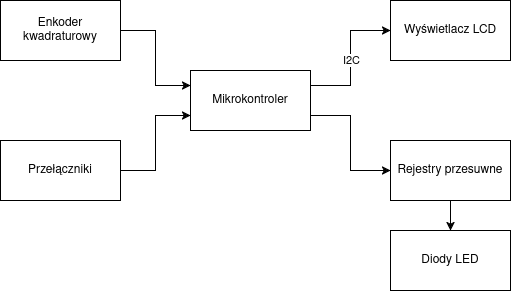
\includegraphics[width=\linewidth]{hardware_diagram.png}
        \caption{Schemat blokowy sprzętowej części zestawu}
        \label{fig:hardware_diagram}
    \end{figure}
    
\subsection{Architektura oprogramowania}

    \subsubsection{Struktura programu}

    Wybrany mikrokontroler RP2040 posiada dostarczane przez producenta SDK dla języka C/C++. W skład zestawu wchodzi szereg
    bibliotek pozwalających na obsługę peryferiów mikrokontrolera. Są to biblioteki niskopoziomowe o niewielkim stopniu abstrakcji.
    Znaczącym ograniczeniem SDK jest niewielka ilość bibliotek do obsługi urządzeń dołączanych do mikrokontrolera.
    W związku z tym do napisania oprogramowania zestawu zdecydowano się wykorzystać framework Arduino \cite{arduino_pico}. Jest to popularne środowisko 
    programistyczne wspierające wiele mikrokontrolerów oparte o język C++. Framework ten dostarcza wysokopoziomowe biblioteki do obsługi
    peryferiów mikrokontrolera. Ze względu na popularność Arduino framework dostępnych jest wiele bibliotek z nim kompatybilnych napisanych
    przez społeczność.
    \par
    Oprogramowanie zestawu podzielono na kilka modułów odpowiadających za poszczególne funkcjonalności zestawu:

    \begin{figure}[H]
        \centering
        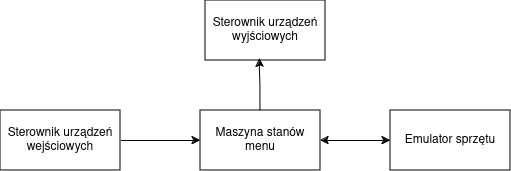
\includegraphics[width=\linewidth]{software_diagram.png}
        \caption{Schemat blokowy oprogramowania zestawu}
        \label{fig:software_diagram}
    \end{figure}

    \subsubsection{Emulacja elementów układu szyny danych}

    \subsubsection{Obsługa peryferiów sprzętowych}

    \subsubsection{Obsługa interfejsu użytkownika}

\end{document}